\section{Experimentos de eficiência}
\label{sec:experimentos-eficiencia}
Nesta Seção, a heurística será aplicada a alguns grafos aleatórios,
com o intuito de averiguar seu custo em tempo à medida que o número de
vértices e arestas do grafo aumenta.

No entanto, como o tempo assintótico é de $O(VE)$, serão feitos
experimentos fixando o número de vértices, e aumentando o número de
arestas.

\subsection{Resultados}

Foram realizados testes com grafos de 1000, 1250, 1500, 1750 e 2000
vértices. Para cada um destes valores, foram gerados grafos com
porcentagens de 10 a 100\% do número máximo de arestas para a
quantidade correspondente de vértices.

Os grafos foram gerados utilizando a ferramenta Python Web Graph
Generator~\cite{cite:pythonwebgenerator}.

A Figura~\ref{fig:vertexchart}
apresenta os tempos para estas execuções.

\begin{figure}[htb!]
\centering
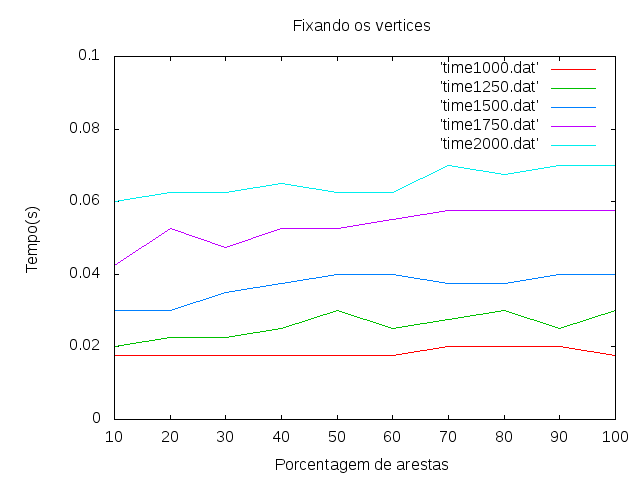
\includegraphics[width=0.7\textwidth]{../dat/plot.png}
\caption{Gráfico fixando o número de vértices}
\label{fig:vertexchart}
\end{figure}

\subsection{Análise}
Pelo gráfico apresentado, nota-se que a influência da variação do
número de arestas pouco influencia no tempo de execução, sendo que a
maior variação é decorrente da variação do número de vértices.

Mais ainda, o tempo foi relativamente baixo, o que sugere que a
heurística se comportaria bem para grafos grandes. Experimentos com
grafos maiores não foram realizados devido às limitações da máquina
utilizada para gerar os grafos: mesmo para os grafos de 2000 vértices,
o gasto de memória para gerar o grafo foi grande, assim como o tempo
gasto para finalizar a geração.
